% SPDX-FileCopyrightText: 2025 Laura Milagros Castro Souto <lcastro@udc.es>
%
% SPDX-License-Identifier: GPL-2.0-or-later

%%%%%%%%%%%%%%%%%%%%%%%%%%%%%%%%%%%%%%%%%%%%%%%%%%%%%%%%%%%%%%%%%%%%%%%%%%%%%%%%
% Preámbulo                                                                    %
%%%%%%%%%%%%%%%%%%%%%%%%%%%%%%%%%%%%%%%%%%%%%%%%%%%%%%%%%%%%%%%%%%%%%%%%%%%%%%%%

\documentclass[11pt,a4paper,titlepage,oneside]{report}

%%% RELACIÓN DE VARIABLES A PERSONALIZAR %%%
% \def\lingua{gal}
%\def\lingua{esp} % descomenta esta liña se redactarás a memoria en español
\def\lingua{eng} % descomenta esta liña se redactarás a memoria en inglés
\def\nome{Jorge Teixeira Crespo}                             % substitúe aquí o teu nome
\def\nomedirectorA{Emilio José Padrón González}              % substitúe aquí o nome de quen dirixe
\def\nomedirectorB{Bruno Cabado Lousa}             % duplica esta liña máis veces se o precisas, cambiando
                                                     % a letra final (A, B, C, D...): úsanse na portada.tex
\def\titulo{Renewing the infrastructure of an association using Open Source tools} % substitúe aquí o título do teu TFG
%\def\titulacion{gced}                               % descomenta esta liña e comenta a seguinte se es estudante do GCED
\def\titulacion{gei}
%\def\mencion{COMPUTACIÓN}                           % descomenta a mención que che corresponda se es estudante do GEI
% \def\mencion{ENXEÑARÍA DO SOFTWARE}
%\def\mencion{ENXEÑARÍA DE COMPUTADORES}
%\def\mencion{SISTEMAS DE INFORMACIÓN}
\def\mencion{TECNOLOXÍAS DA INFORMACIÓN}

%\def\renomearcadros{si} % descomenta esta liña se redactas a memoria en español e prefires que
                         % os "cuadros" e o "índice de cuadros" se renomeen
                         % a "tablas" e "índice de tablas" respectivamente

\usepackage{estilo_tfg}

% Lista de paquetes potencialmente interesantes (uso baixo demanda)

% \usepackage{alltt}       % proporciona o entorno alltt, semellante a verbatim pero que respecta comandos
% \usepackage{enumitem}    % permite personalizar os entornos de lista
% \usepackage{eurofont}    % proporciona o comando \euro
\usepackage{float}       % permite máis opcións para controlar obxectos flotantes (táboas, figuras)
% \usepackage{hhline}      % permite personalizar as liñas horizontais en arrays e táboas
  \usepackage{longtable}   % permite construir táboas que ocupan máis dunha páxina
% \usepackage{lscape}      % permite colocar partes do documento en orientación apaisada
% \usepackage{moreverb}    % permite personalizar o entorno verbatim
  \usepackage{multirow}    % permite crear celdas que ocupan varias filas da mesma táboa
% \usepackage{pdfpages}    % permite insertar ficheiros en PDF no documento
% \usepackage{rotating}    % permite diferentes tipos de rotacións para figuras e táboas
% \usepackage{subcaption}  % permite a inclusión de varias subfiguras nunha figura
% \usepackage{tabu}        % permite táboas flexibles
% \usepackage{tabularx}    % permite táboas con columnas de anchura determinada

% Paquetes engadido a maiores
\usepackage[edges]{forest}

%%%%%%%%%%%%%%%%%%%%%%%%%%%%%%%%%%%%%%%%%%%%%%%%%%%%%%%%%%%%%%%%%%%%%%%%%%%%%%%%
% Corpo                                                                        %
%%%%%%%%%%%%%%%%%%%%%%%%%%%%%%%%%%%%%%%%%%%%%%%%%%%%%%%%%%%%%%%%%%%%%%%%%%%%%%%%

\begin{document}

 %%%%%%%%%%%%%%%%%%%%%%%%%%%%%%%%%%%%%%%%
 % Preliminares do documento            %
 %%%%%%%%%%%%%%%%%%%%%%%%%%%%%%%%%%%%%%%%

 % SPDX-FileCopyrightText: 2025 Laura Milagros Castro Souto <lcastro@udc.es>
%
% SPDX-License-Identifier: GPL-2.0-or-later

\begin{titlepage}
  
  \hspace*{128pt}
  \textcolor{udcpink}{{\fontencoding{T1}\fontfamily{phv}\selectfont Facultade de Informática}}\\[-32pt]

  \begin{center}
    \includegraphics[scale=0.3]{imaxes/udc}\\[25pt]

    {\large TRABALLO FIN DE GRAO \\
            \nometitulacion \\
            \nomemencion } \\[10pt]

    \carimbo \\[25pt]

    \begin{huge}
      \begin{spacing}{1.3}
        \bfseries \titulo
      \end{spacing}
    \end{huge}
  \end{center}
  
  \vfill
  
  \begin{flushright}
    {\large
    \begin{tabular}{ll}
      {\bf Student:} & \nome \\
      {\bf Direction:} & \nomedirectorA \\
                     & \nomedirectorB \\ % duplica esta liña máis veces se o precisas, cambiando
                                           % a letra final (A, B, C, D...); define eses nomes no memoria_tfg.tex
    \end{tabular}}
  \end{flushright}
  \rightline{A Coruña, \datasimple.}
\end{titlepage}

 \dedicatoria{Dedicatoria} % escribe neste comando o teu texto de dedicatoria
 \paxinaenbranco
 \begin{agradecementos}
 \blindtext                % substitúe este comando polo teu texto de agradecementos
 \end{agradecementos}
 %%%%%%%%%%%%%%%%%%%%%%%%%%%%%%%%%%%%%%%%%%%%%%%%%%%%%%%%%%%%%%%%%%%%%%%%%%%%%%%%

\pagestyle{empty}
\begin{abstract}
  \blindtext % substitúe este comando polo resumo do teu TFG
             % na lingua principal do documento (tipicamente: galego)

  \vspace*{25pt}
  \begin{segundoresumo}
    \blindtext % substitúe este comando polo resumo do teu TFG
               % na lingua secundaria do documento (tipicamente: inglés)
  \end{segundoresumo}
\vspace*{25pt}
% SPDX-FileCopyrightText: 2025 Laura Milagros Castro Souto <lcastro@udc.es>
%
% SPDX-License-Identifier: GPL-2.0-or-later

\begin{multicols}{2}
\begin{description}
\item [\palabraschaveprincipal:] \mbox{} \\[-20pt]
  \blindlist{itemize}[7] % substitúe este comando por un itemize
                         % que relacione as palabras chave
                         % que mellor identifiquen o teu TFG
                         % no idioma principal da memoria (tipicamente: galego)
\end{description}
\begin{description}
\item [\palabraschavesecundaria:] \mbox{} \\[-20pt]
  \blindlist{itemize}[7] % substitúe este comando por un itemize
                         % que relacione as palabras chave
                         % que mellor identifiquen o teu TFG
                         % no idioma secundario da memoria (tipicamente: inglés)
\end{description}
\end{multicols}

\end{abstract}
\pagestyle{fancy}

%%%%%%%%%%%%%%%%%%%%%%%%%%%%%%%%%%%%%%%%%%%%%%%%%%%%%%%%%%%%%%%%%%%%%%%%%%%%%%%%


 \pagenumbering{roman}
 \setcounter{page}{1}
 \bstctlcite{IEEEexample:BSTcontrol}

 \tableofcontents
 \listoffigures
 \listoftables
 \clearpage
 
 \pagenumbering{arabic}
 \setcounter{page}{1}

 %%%%%%%%%%%%%%%%%%%%%%%%%%%%%%%%%%%%%%%%
 % Capítulos                            %
 %%%%%%%%%%%%%%%%%%%%%%%%%%%%%%%%%%%%%%%%

 % SPDX-FileCopyrightText: 2025 Jorge Teixeira Crespo <jorge.teixeira@udc.es>
%
% SPDX-License-Identifier: GPL-2.0-or-later

\chapter{Introduction}
\label{chap:introduction}

\lettrine{I}{n} the current digital era, nearly every organization depends on a solid technological infrastructure to operate effectively. From internal coordination to external communication, from document management to compliance with legal obligations, many day-to-day tasks rely on tools hosted online or managed digitally. This trend has made IT infrastructure not only a convenience but a fundamental requirement.

For non-profit associations and student communities, the challenge is particularly complex. These entities often lack dedicated IT staff and operate with minimal budgets, yet they are expected to manage technological services. Moreover, many of them, especially those driven by ideological commitments, reject proprietary or SaaS solutions in favor of Free and Open Source Software (FOSS). This decision aligns with their values but often increases the burden of system maintenance and security.

A typical association today might need to run one or more websites, handle mailing lists, share files securely, issue invoices under national tax regulations, and coordinate internal communication. These needs must be met through tools that are easy to maintain, well-documented, and adaptable to the association's size and structure. However, in practice, infrastructure is often built incrementally over many years by different people, leading to heterogeneous, outdated, and fragile systems.

This work addresses these challenges by analyzing the typical software needs of non-profit associations and proposing practical guidelines for building and maintaining the required infrastructure. In addition to identifying common services and technical requirements, we also study the case of a long-standing real-world association, which has been operating for more than 25 years. This provides an opportunity to examine the problems that often arise when infrastructure grows organically over time: ad-hoc patches, short-term decisions that eventually become permanent, and the resulting accumulation of technical debt. We discuss the process of transitioning from such a fragmented system to a more rational, maintainable, and future-proof infrastructure.


\section{Context and motivation}

GPUL (Grupo de Programadores e Usuarios de Linux) \cite{gpul-web} provides a concrete example of such an organization, with characteristics that make its case especially notable. Founded in 1998 in A Coruña, GPUL promotes Free Software and technical education through community events, workshops, and conferences. Closely tied to the field of computer engineering and to the Faculty of Computer Science at the Universidade da Coruña, many of its members are current or former students, as well as professionals, with a strong technical background. This makes it easier to adopt and maintain open-source infrastructure, and also turns the infrastructure itself into a valuable learning environment. The association's long-standing commitment to the principles of software freedom drives it to self-host most of its services using libre tools, an approach that aligns with its values but also amplifies the common challenges of volunteer-managed systems.

Today, GPUL's services are distributed across two aging servers, GPULINO and GPULON, which run critical tools like an old Nextcloud instance for internal documentation and a Mailman 2 server that manages our mailing lists. These machines suffer from poor documentation, lack of backups, and limited monitoring, issues that are worsened by the fact that the board of the association changes every two years, often leaving gaps in technical knowledge. As current president, we have had to deal with several crises caused by this fragile setup.

One example was when our email redirection system, which uses manual redirects for addresses under the gpul.org domain, caused our messages to be flagged as spam, affecting communication with sponsors and participants during events. Another incident occurred shortly before the financial quarter deadline, when our Nextcloud instance went down due to a full disk caused by unrotated logs. Without documentation or clear monitoring, it took four days and help from former members and our hosting provider to bring the system back online, almost making us miss administrative deadlines with possible financial penalties.

Faced with this situation, we decided to renew GPUL's infrastructure entirely. The goal is not only to modernize the services but also to ensure they are well-documented, sustainable, and easy to maintain by future teams. In evaluating options, we considered managed services and commercial tools but discarded most of them due to their incompatibility with our philosophy or excessive costs. Among the various tools considered, Odoo \cite{odoo-web} stood out as a cloud-capable open-source platform that can also be self-hosted. We have chosen to self-host it and use it primarily for invoicing, particularly to comply with Spain's new \gls{verifactu} regulations \cite{boe-a-2024-22138}. While invoicing is our main use case for now, Odoo's modular and extensible architecture leaves the door open to adopting other features in the future if needed.

For the rest of the stack, our approach has been to improve and modernize the existing FOSS tools already in use within the association. This includes migrating from Mailman 2 to Mailman 3 integrated with HyperKitty \cite{hyperkitty-web}, which improves usability and provides a web interface for list archives, and upgrading Nextcloud to a modern version with better backup and monitoring systems. For the email service, given its complexity and importance, we are still considering whether to keep it self-hosted or switch to a trusted external provider, always balancing autonomy with reliability.
This work documents the process of renewing GPUL's infrastructure with a focus on sustainability, maintainability, and alignment with our values. It includes an in-depth analysis of the current systems, the design of the new infrastructure, the rationale behind each technological choice, and the steps taken during migration. The aim is to leave behind a robust foundation and clear documentation for future contributors, ensuring that our commitment to Free Software is matched by reliable, modern, and resilient infrastructure.

\section{Objectives}

Given these critical challenges, the objectives of this project are to:

\begin{itemize}
    \item Modernize and simplify GPUL's infrastructure to ensure long-term maintainability.
    \item Replace outdated services (like Mailman 2 and legacy Nextcloud) with modern, modular open-source solutions.
    \item Implement proper documentation to facilitate knowledge transfer and reduce dependency on individual members.
    \item Enhance the reliability, performance, and security of critical infrastructure services, incorporating robust backup solutions.
    \item Empower new contributors with clear processes and documentation, ensuring continuity and sustainability.
    \item Ensure alignment with GPUL's foundational values of openness and community-driven development.
\end{itemize}

The priority lies in modernization, simplification, and thorough documentation, underpinned by improved security and reliable backup procedures.

\section{Thesis Structure}

TBD.

 % SPDX-FileCopyrightText: 2025 Jorge Teixeira Crespo <jorge.teixeira@udc.es>
%
% SPDX-License-Identifier: GPL-2.0-or-later

\chapter{Project Methodology}
\label{chap:project-methodology}

\lettrine{T}{ransparency}, reproducibility, and effective collaboration through open tools and platforms form the foundation of this thesis's development methodology. Given the diverse schedules and availability constraints of those involved, asynchronous communication has been explicitly chosen as the primary mode of interaction. This approach facilitates flexibility, allows thorough peer review, and accommodates the varying responsibilities of project participants.

\section{Open Development}

The entire thesis development is conducted openly within a public GitHub repository.\footnote{\url{https://github.com/jorgeteixe/thesis}} All thesis source files, configurations, and relevant documentation are version-controlled, publicly accessible, and managed using a pull request workflow. This enables structured peer review of both technical decisions and thesis content. Continuous integration is automated through GitHub Actions, which generate the thesis PDF document upon every change. This approach ensures immediate feedback, reproducibility, and simplifies collaboration with supervisors.

Throughout the thesis, all configurations, scripts, and tools subject to being open-sourced are either already publicly available or will be made publicly available.\footnote{\url{https://github.com/gpul-org}} Official documentation will be openly hosted on the association's website, providing comprehensive guidance and ensuring traceability and accountability for all project-related decisions. This open and documented approach not only supports transparency but also creates a valuable resource for future students, contributors, and maintainers.

\section{Planning and Methodology}

\lettrine{T}{he} planning for this thesis follows a structured approach inspired by the classic \emph{Waterfall} methodology. This choice is primarily driven by the clear and sequential dependencies between project phases, which naturally fit a linear model.

The initial planning stage involves a comprehensive forensic analysis of the existing infrastructure, clearly identifying active services, their usage, and existing limitations. The subsequent phase, state-of-the-art analysis, builds directly upon this initial assessment. Each required service is systematically evaluated through practical testing, informing both technological decisions and preliminary resource estimates.

In parallel, potential hosting providers are to be explored. Although initial resource requirements can be estimated after evaluating candidate technologies, final confirmation depends on the definitive technology selection, establishing a clear dependency between these tasks.

Implementation is planned to proceed sequentially due to explicit task dependencies: setting up the hosting provider account, installing the base system, configuring container environments, and deploying selected services in a predetermined order. Documentation and thesis writing activities will run concurrently to ensure comprehensive records of the processes.

Finally, a structured migration and handover phase is planned after thesis submission. This phase will ensure operational readiness and facilitate effective knowledge transfer to future maintainers, reinforcing sustainability.

A Gantt chart illustrating these phases is shown in Figure~\ref{fig:gantt-planned}, spanning a four-month period from March 1st to the beginning of July.

\begin{figure}[H]
  \centering
  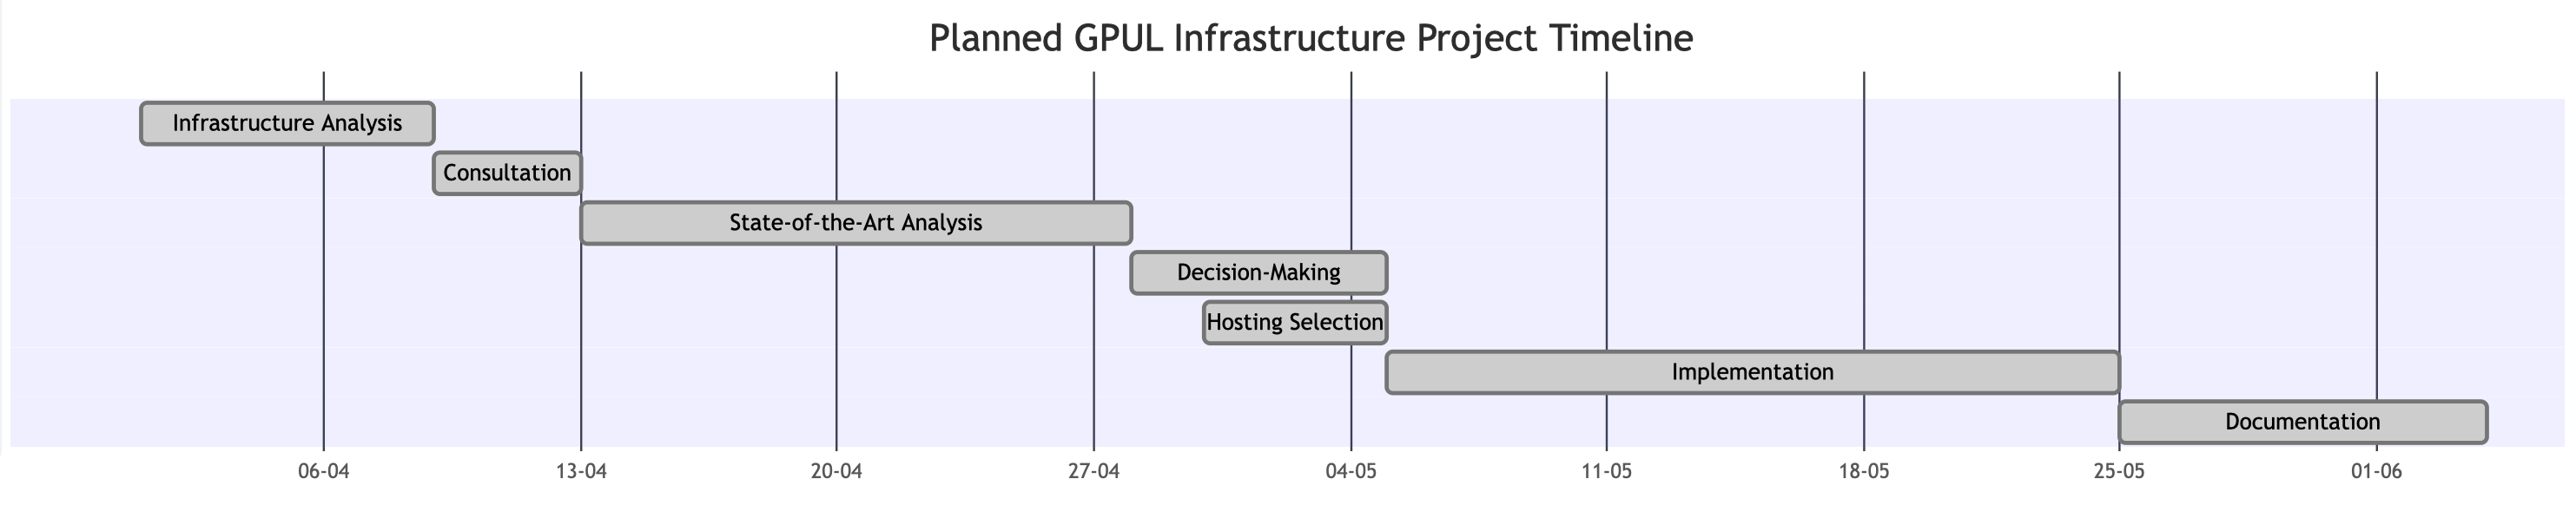
\includegraphics[width=1\textwidth]{imaxes/gantt-planned.png}
  \caption{Gantt chart illustrating the planned project phases.}
  \label{fig:gantt-planned}
\end{figure}

\subsection*{Phases}

\begin{enumerate}
  \item \textbf{Initial Infrastructure Analysis}\\
  Independent analysis of the legacy servers \texttt{GPULINO} and \texttt{GPULON}. Task included service inspection and identification of required services.\\
  \emph{Estimated duration: \(\sim 50\)~hours.}

  \item \textbf{Consultation and Requirements Gathering}\\
  Discussions with current and former board members to define required services.\\
  \emph{Estimated duration: \(\sim 20\)~hours.}

  \item \textbf{State-of-the-Art Analysis and Testing}\\
  Research of candidate solutions and practical trials on a self-hosted test environment.\\
  \emph{Estimated duration: \(\sim 60\)~hours.}

  \item \textbf{Technology Selection}\\
  Consolidation of testing results with the board and thesis supervisor to agree on the software stack.\\
  \emph{Estimated duration: \(\sim 20\)~hours.}

  \item \textbf{Hosting Provider Selection}\\
  Meetings with local providers and evaluation of alternatives. Carried out in parallel with the previous phase.\\
  \emph{Estimated duration: \(\sim 15\)~hours.}

  \item \textbf{Implementation}\\
  Sequential deployment of the new infrastructure: provisioning the environment, installing Incus, configuring containers, and deploying the selected services.\\
  \emph{Estimated duration: \(\sim 90\)~hours.}

  \item \textbf{Documentation and Thesis Writing}\\
  Documentation of procedures and preparation of the thesis document.\\
  \emph{Estimated duration: \(\sim 30\)~hours.}

\end{enumerate}

\subsection*{Relevant Deviations}

While the overall structure of the project largely followed the initial plan, several key deviations occurred, primarily impacting the project timeline. Most notably, all phases commenced approximately one week later than initially anticipated, leading to incremental delays in subsequent stages.

The primary delay arose during the hosting provider selection phase. Initial conversations suggested an imminent agreement; however, the final proposal did not meet the association's expectations in terms of value and resource allocation. This unexpected outcome necessitated reopening discussions and evaluating alternative options, significantly pushing back the start of the implementation phase.

Furthermore, work was completely halted between June 12th and 15th due to organizational duties for the AtlanticaConf event. This interruption occurred during a peak implementation period, compounding the initial delays and further extending the project timeline.

Due to these compounded delays, the implementation phase had to be adjusted. Instead of fully migrating all services immediately, a decision was made to thoroughly test and validate migration procedures, ensuring readiness without performing the complete migrations. The final domain migrations and service transitions were intentionally postponed until after this thesis submission.

To effectively facilitate this postponed migration, an already scheduled on-site retreat, originally planned for general association maintenance and fostering new ideas and future activities, was partially repurposed. This intensive weekend will now also include migration tasks, with the in-person communication enabling faster account provisioning and smoother transitions compared to the usual asynchronous exchanges. The direct face-to-face interactions will streamline knowledge transfer between current, historical, and newly active board members, avoiding the delays inherent to remote communication. Ultimately, this adjustment addressed the tight thesis submission deadline while promoting long-term infrastructure sustainability through enhanced collective involvement and communication.

Figure~\ref{fig:gantt-real} illustrates the revised project timeline, which reflects the initial one-week offset and the subsequent delays. As a result, the implementation phase extended into early July, with final migrations deferred until after the thesis submission.

\begin{figure}[H]
  \centering
  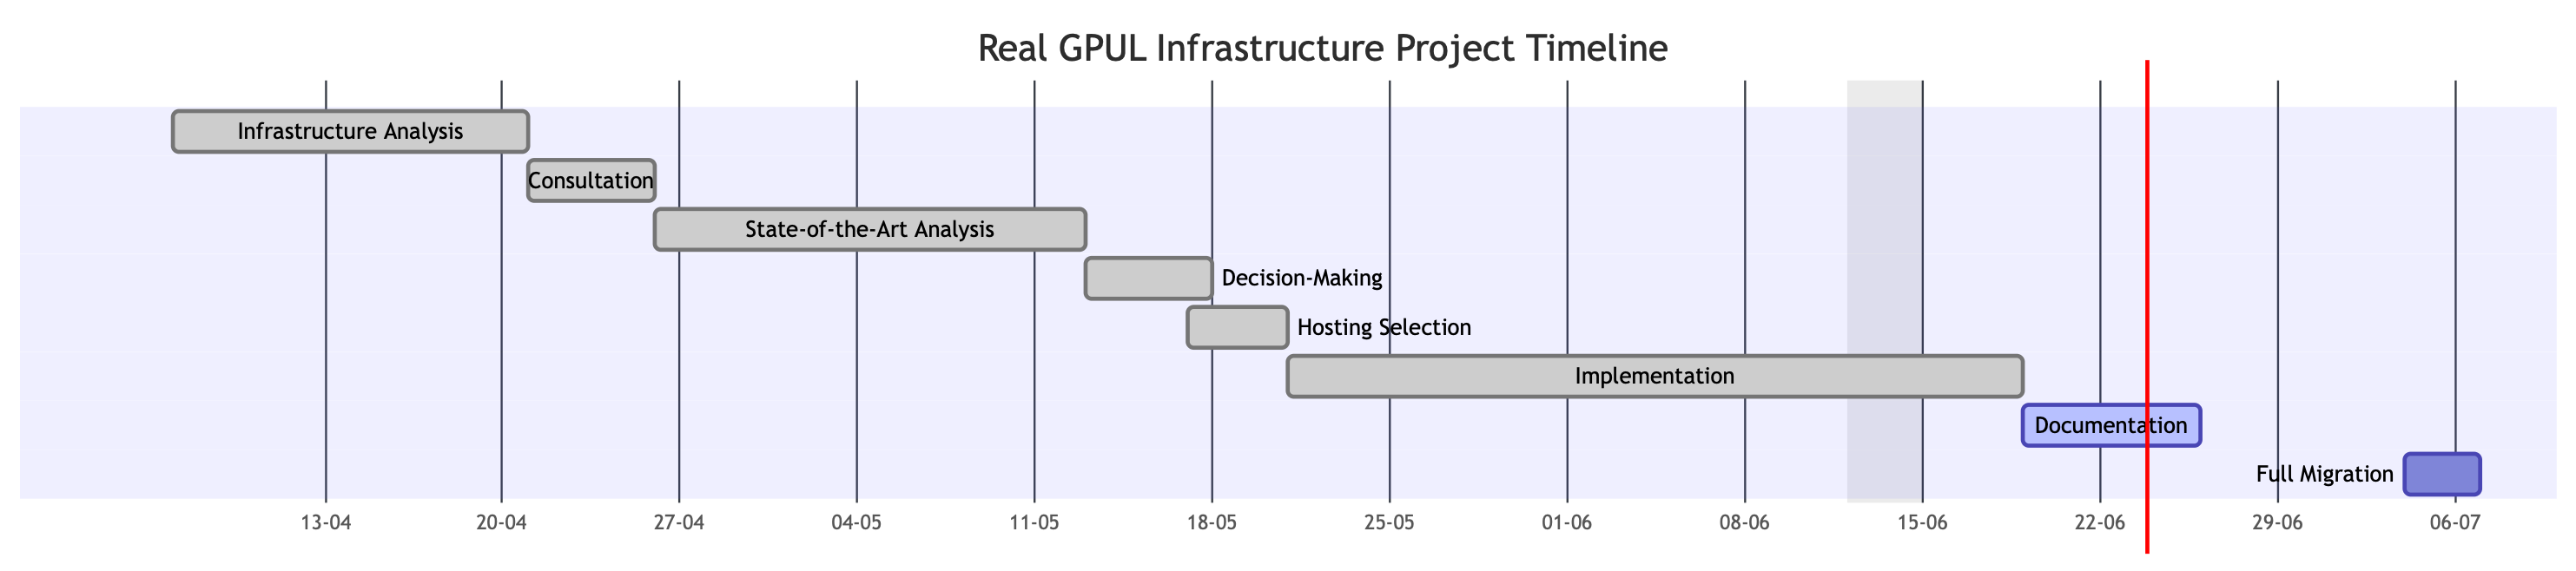
\includegraphics[width=1\textwidth]{imaxes/gantt-real.png}
  \caption{Gantt chart illustrating the real project phases.}
  \label{fig:gantt-real}
\end{figure}

\section{Cost Estimation}

Although this project was conducted under the umbrella of a volunteer-driven nonprofit organization, certain infrastructure, equipment, and labor costs can be roughly estimated to provide context on the real-world value of the work.

\subsection*{Equipment and Resources}

The development and testing work was carried out using a personal laptop and a repurposed self-hosted desktop PC:

\begin{itemize}
  \item \textbf{Laptop (development machine)}: \(\sim 1\,200€\), mid-range Linux-compatible machine.
  \item \textbf{Test server}: no acquisition cost, reused legacy hardware from prior GPUL use.
  \item \textbf{Domain name} (\texttt{gpulux.org}): \(\sim 10€\)/year.
  \item \textbf{Production server}: costs are detailed in Chapter~\ref{chap:hosting-provider}.
\end{itemize}

\subsection*{Human Resources and Labor Value}

While no direct financial compensation was involved, estimating the cost of human labor provides perspective on the real investment made, especially considering that all three individuals involved (the author and two supervisors) are not only members of the association, but also active or former board members with a high level of involvement and responsibility.

\begin{itemize}
  \item \textbf{System Administration and Infrastructure Work}: Based on the 2024 Manfred Developer Report~\cite{manfred-salary-guide}, see Figure~\ref{fig:salary-chart}, the most common salary bracket for SysAdmin roles is \textbf{€30-40K}. This work cannot be considered entry-level, as the author has over five years of professional experience and holds prior technical qualifications. Assuming a midpoint of \textbf{€35\,000} for a full-time equivalent, and with an estimated dedication of 300 hours, the work carried out corresponds to a market value of approximately \(\sim 5\,800€\).

  \item \textbf{Supervision and Guidance}: For technical supervisors involved in infrastructure or SRE roles, the most common salary bracket is higher: \textbf{€40-50K}. Using a midpoint estimate of \textbf{€45\,000} per year, their involvement (estimated 8-12 hours per supervisor) corresponds to an approximate market value of \(\sim 450€\) in total.
\end{itemize}

\begin{figure}[H]
  \centering
  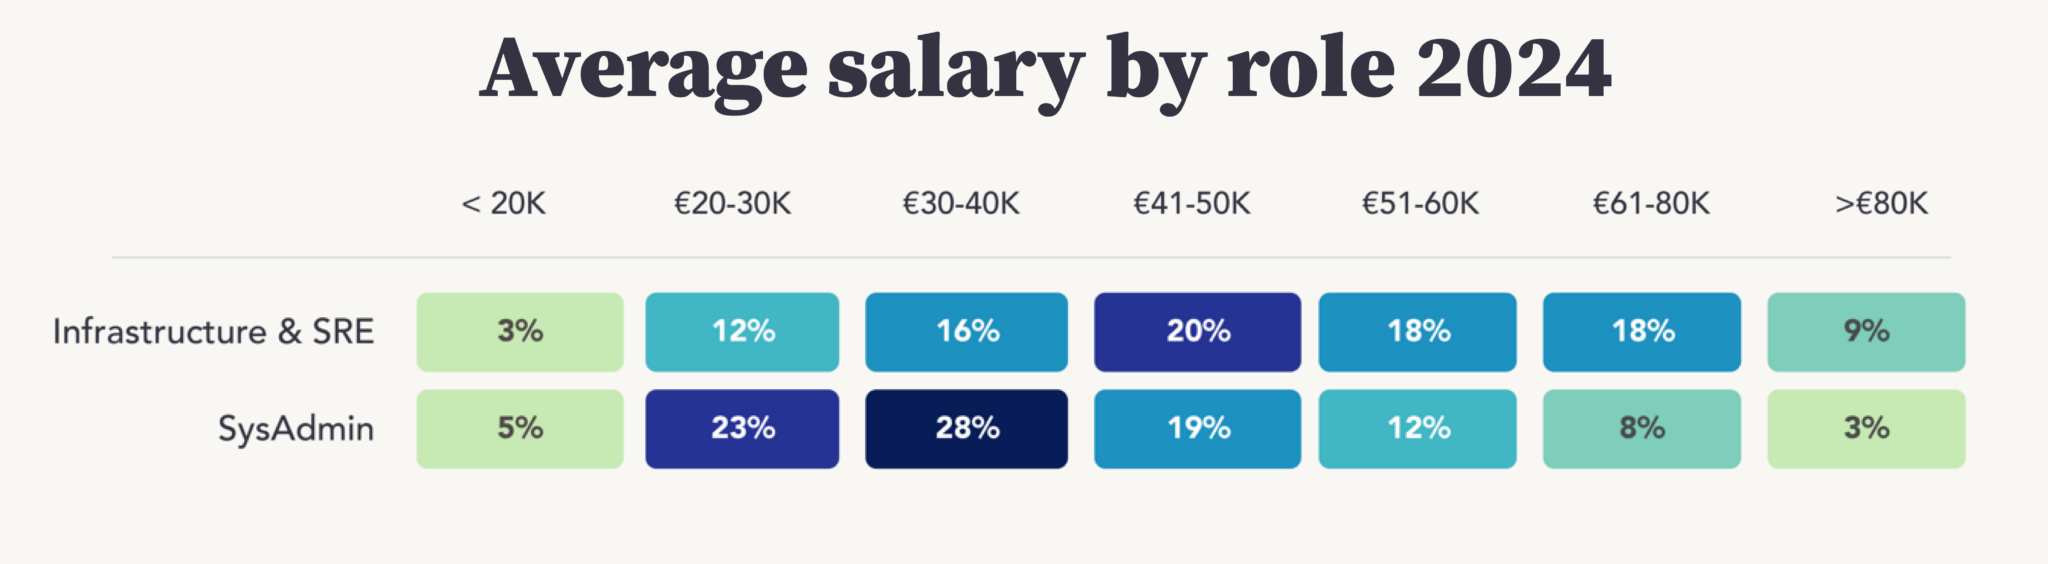
\includegraphics[width=0.8\textwidth]{imaxes/salary-chart.png}
  \caption{Average salary distribution in Spain by role.}
  \label{fig:salary-chart}
\end{figure}

These estimates illustrate that while the project was executed in a volunteer context, the real value of the technical and organizational contributions exceeds \(\sim 6\,000€\). This reinforces the importance of properly valuing community infrastructure efforts and documenting them for long-term sustainability.

 % SPDX-FileCopyrightText: 2025 Jorge Teixeira Crespo <jorge.teixeira@udc.es>
%
% SPDX-License-Identifier: GPL-2.0-or-later

\chapter{Current Infrastructure Analysis}
\label{chap:current-infrastructure}

\lettrine{A}{n} in-depth analysis of GPUL's current server infrastructure focuses on the two legacy servers: GPULINO and GPULON. These servers host critical services but also pose significant operational and maintenance challenges. GPULINO, created on November 3, 2011, and GPULON, launched on January 17, 2016, have remained largely unchanged since their deployment. The chapter reviews their specifications, configurations, and highlights key issues such as outdated software, inconsistent backup strategies, and the lack of proper documentation. It also discusses the impact of these limitations on GPUL's operations, underlining the urgent need for a comprehensive infrastructure renewal.

\section{GPULINO Server Analysis}

GPULINO is hosted with Gandi, located in their Paris, France (SD3 datacenter). It runs Debian GNU/Linux 8 (Jessie), which is significantly outdated. Its official End-of-Life (EOL) was June 17, 2018, and Long-Term Support (LTS) concluded on June 30, 2020.

\subsection*{Technical Specifications}

GPULINO is a legacy virtual machine that remains in active use within the association's infrastructure. Provisioned in 2011, it has undergone minimal changes since its deployment. The table below summarizes its key specifications, which reflect the outdated and limited nature of the system. These constraints have direct implications for performance, maintenance, and security.

\begin{table}[H]
  \centering
  \rowcolors{2}{white}{udcgray!25}
  \caption{GPULINO Server Specifications}
  \label{tab:gpulino_specs}
  \begin{tabular}{ll}
    \rowcolor{udcpink!25}
    \textbf{Specification} & \textbf{Details} \\
    \hline
    CPU & 1 core \\
    RAM & 640 MB \\
    Storage & 3 x 10 GB volumes \\
    Monthly Cost & €13.09 \\
    IPv4 & 95.142.163.196 \\
    IPv6 & 2001:4b98:dc0:47:216:3eff:fe56:1785 \\
    OS & Debian GNU/Linux 8 (Jessie, EOL) \\
  \end{tabular}
\end{table}

\subsection*{Filesystem Structure}

GPULINO uses three independent 10 GB volumes provided by the hosting provider. These are mounted as root (\verb|/|), data (\verb|/srv/srv_gpulino|), and backup (\verb|/srv/backup_gpulino|). Their current usage is visualized in Figure~\ref{fig:gpulino_disk_usage}.

\begin{figure}[H]
  \centering
  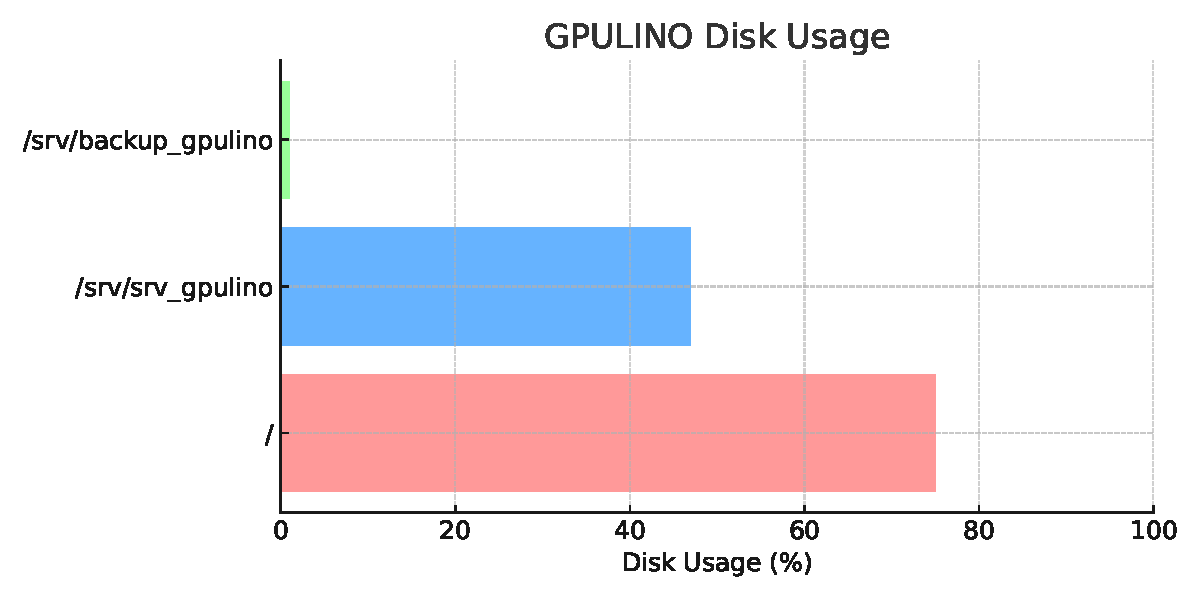
\includegraphics[width=0.7\textwidth]{figuras/gpulino_disk_usage.pdf}
  \caption{Disk usage across GPULINO volumes.}
  \label{fig:gpulino_disk_usage}
\end{figure}

While the root filesystem is nearing critical usage (~75\%), the backup volume remains largely underutilized (~1\%), showcasing the lack of backup strategy.

\subsection*{User Access and Management}

The server maintains several user accounts, with varying levels of activity. Table \ref{tab:gpulino_users} shows the most relevant user logins:

\begin{table}[H]
  \centering
  \rowcolors{2}{white}{udcgray!25}
  \caption{GPULINO Active User Accounts (sorted by creation date)}
  \label{tab:gpulino_users}
  \begin{tabular}{ll}
    \rowcolor{udcpink!25}
    \textbf{Username} & \textbf{Last Login} \\
    \hline
    adm***** & September 26, 2020 \\
    tsa***** & September 27, 2024 \\
    ssa***** & January 27, 2024 \\
    mar***** & February 19, 2014 \\
    cas***** & March 18, 2017 \\
    che***** & April 24, 2019 \\
    tei***** & January 19, 2025 \\
  \end{tabular}
\end{table}

\subsection*{Active Services and Usage Details}

The server hosts several critical services:
\begin{itemize}
    \item Apache2 Web Server
    \item Exim4 Mail Transport Agent
    \item Mailman 2 (for mailing lists)
    \item MySQL (database server, supporting Mailman)
    \item SSH (Secure Shell)
\end{itemize}

Although these services were known to be active, GPULINO lacked formal documentation. A manual inspection of the server's filesystem and configuration files revealed various hosted domains, tools, and historical content.

The Apache configuration included several virtual hosts pointing to subdomains, some of which were no longer functional. Others still displayed static content or redirected to internal projects.

\begin{table}[H]
  \centering
  \rowcolors{2}{white}{udcgray!15}
  \caption{Web domains served by Apache on GPULINO}
  \label{tab:gpulino_apache_domains}
  \begin{tabular}{ll}
    \rowcolor{udcpink!25}
    \textbf{Domain} & \textbf{Notes} \\
    \hline
    \texttt{planet.gpul.org} & Hosts a blog or webpage \\
    \texttt{old.gpul.org} & Returns a PHP error \\
    \texttt{stuff.gpul.org} & Hosts a webpage \\
    \texttt{dudesconf.org} & Hosts a webpage (some links broken) \\
    \texttt{junoffice.gpul.org} & Returns an empty page \\
    Other domains & Serve the default Apache welcome page \\
  \end{tabular}
\end{table}

These domains pointed to directories inside \texttt{/var/www}, which contained a variety of static and symlinked content likely tied to past events, services, or internal documentation.

\begin{table}[H]
  \centering
  \rowcolors{2}{white}{udcgray!15}
  \caption{Apache web directories found under \texttt{/var/www}}
  \label{tab:gpulino_www_dirs}
  \begin{tabular}{ll}
    \rowcolor{udcpink!25}
    \textbf{Directory} & \textbf{Description} \\
    \hline
    apache-default & Default Apache content \\
    artwork & Publicly accessible artwork files \\
    drupal & Linked to \texttt{/var/www/gpul.org/drupal} \\
    dudesconf & Hosts content for dudesconf.org \\
    estatutos & Organizational rules or statutes \\
    etherpad-lite & Likely collaborative editor \\
    eventostuff & Linked to \verb|/srv/srv_gpulino/eventos| \\
    gallery2 & Public gallery \\
    gpul-latex & LaTeX-related files \\
    gpul.org & Main content for GPUL \\
    gpul.org-eventos & Event-specific content \\
    guademy & Linked to \verb|/srv/srv_gpulino/www/guademy/| \\
    indico & Linked to \verb|/srv/srv_gpulino/indico| \\
    junoffice & Content for junoffice.gpul.org \\
    labs.gpul.org & Lab-related subdomain \\
    piwik & Web analytics platform \\
    planet.gpul.org & Static site content \\
    rexistro.labs.gpul.org & Registry or logs \\
    votologo & Likely a voting tool \\
  \end{tabular}
\end{table}

Mailman was configured to manage mailing lists under the \texttt{lists.gpul.org} domain, using a CGI interface and Apache redirection rules. The configuration was minimal but functional.

\begin{table}[H]
  \centering
  \rowcolors{2}{white}{udcgray!15}
  \caption{Mailman service details on GPULINO}
  \label{tab:gpulino_mailman}
  \begin{tabular}{ll}
    \rowcolor{udcpink!25}
    \textbf{Parameter} & \textbf{Value} \\
    \hline
    Domain & \texttt{lists.gpul.org} \\
    VirtualHost & Redirects root to \texttt{/cgi-bin/mailman/listinfo} \\
    CGI Path & \texttt{/usr/lib/cgi-bin/} \\
    DocumentRoot & \texttt{/var/www/} \\
    Admin Email & \texttt{mailman@lists.gpul.org} \\
  \end{tabular}
\end{table}

The server also ran a Git daemon that served multiple repositories under a single base path. These were accessible via the \texttt{git://} protocol and configured to run from a root-owned script.

\begin{table}[H]
  \centering
  \rowcolors{2}{white}{udcgray!15}
  \caption{Git daemon configuration details}
  \label{tab:gpulino_git_daemon}
  \begin{tabular}{ll}
    \rowcolor{udcpink!25}
    \textbf{Parameter} & \textbf{Value} \\
    \hline
    Startup Script & \texttt{/root/git-daemon} \\
    Base Path & \verb|/srv/srv_gpulino/git/repositories/| \\
  \end{tabular}
\end{table}

\noindent
\textbf{Git Daemon Command:}

\begin{lstlisting}[language=sh]
/usr/bin/git-daemon \
  --user=git --group=git \
  --verbose \
  --reuseaddr \
  --base-path=/srv/srv_gpulino/git/repositories/ \
  /srv/srv_gpulino/git/repositories/
\end{lstlisting}

\begin{table}[H]
  \centering
  \rowcolors{2}{white}{udcgray!15}
  \caption{Git repositories hosted}
  \label{tab:gpulino_git_repos}
  \begin{tabular}{ll}
    \rowcolor{udcpink!25}
    \textbf{Repository} & \textbf{Description} \\
    \hline
    \texttt{actas.git} & Meeting minutes \\
    \texttt{certificado-asistencia.git} & Attendance certificates \\
    \texttt{cuentas.git} & Financial records \\
    \texttt{gitosis-admin.git} & Git access management \\
    \texttt{gpul-estatutos.git} & Organization statutes \\
    \texttt{manual-latex.git} & LaTeX training material \\
    \texttt{mem-dudesconf.git} & DudesConf report \\
    \texttt{parte-gasto.git} & Expense reports \\
    \texttt{subvencion-udc-2011.git} & UDC grant files (2011) \\
  \end{tabular}
\end{table}

These findings illustrate the range of active uses the server had, many of which were not documented but still functional at the time of analysis. They also reflect the historical depth and variety of GPUL's activities over the years.

\section{GPULON Server Analysis}

GPULON is hosted with Kimsufi and configured as a KS-4C server running Debian GNU/Linux 11 (Bullseye).

\subsection*{Technical Specifications}

\begin{table}[H]
  \centering
  \rowcolors{2}{white}{udcgray!25}
  \caption{GPULON Server Specifications}
  \label{tab:gpulon_specs}
  \begin{tabular}{ll}
    \rowcolor{udcpink!25}
    \textbf{Specification} & \textbf{Details} \\
    \hline
    CPU & Intel i5-2300 \\
    RAM & 16 GB \\
    Storage & 1 x 2TB HDD \\
    Monthly Cost & €30.60 \\
    IPv4 & 91.121.65.91 \\
    OS & Debian GNU/Linux 11 (Bullseye) \\
  \end{tabular}
\end{table}

\subsection*{Filesystem Structure}

GPULON has a single 2 TB physical disk, divided into logical volumes for \texttt{/home}, \texttt{/var/lib/docker}, and the root filesystem (\texttt{/}). This setup is visualized in Figure~\ref{fig:gpulon_disk_usage}.

\begin{figure}[H]
  \centering
  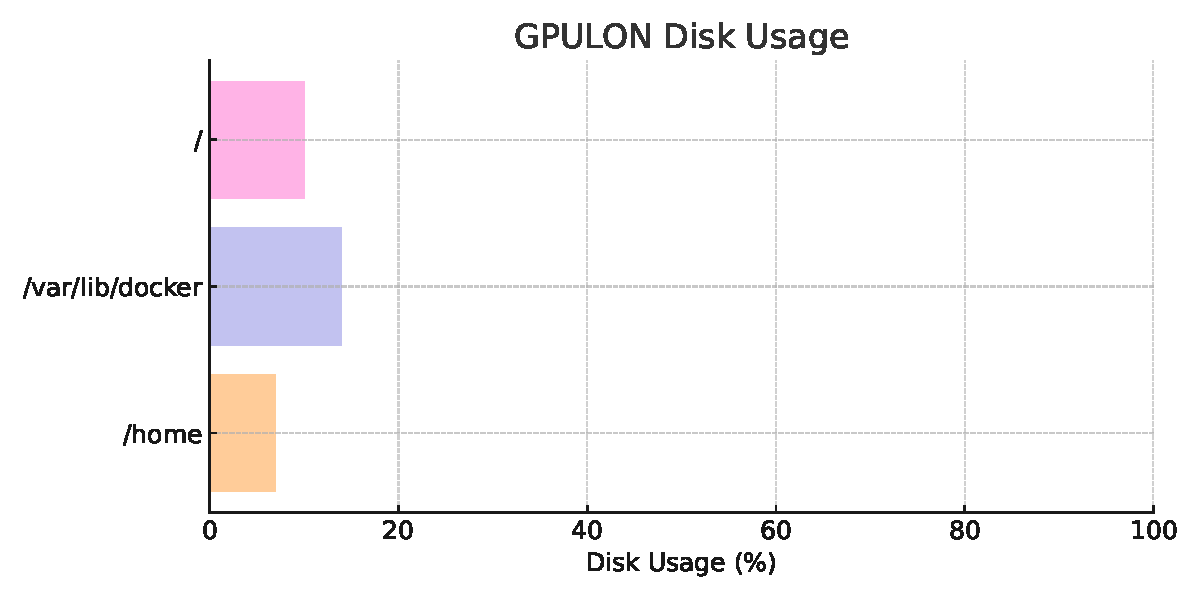
\includegraphics[width=0.7\textwidth]{figuras/gpulon_disk_usage.pdf}
  \caption{Disk usage across GPULON logical volumes after reallocation.}
  \label{fig:gpulon_disk_usage}
\end{figure}

Originally, the Docker directory (\texttt{/var/lib/docker}) had been restricted to approximately 450 GB and became rapidly saturated, primarily due to logs generated by long-running containerized services. One Nextcloud log file alone exceeded 250 GB.

This issue caused an operational incident that affected system stability. Resolving it involved manually deleting the oversized log and reallocating disk space to expand the Docker volume.

The updated logical volume allocation now stands as follows:

\begin{itemize}
    \item \texttt{/home} — 272 GB (7\% usage)
    \item \texttt{/var/lib/docker} — 1.5 TB (14\% usage)
    \item Root filesystem (\texttt{/}) — 58 GB (10\% usage)
\end{itemize}

This reallocation has significantly improved headroom for service logs and application data, reducing the risk of similar incidents in the future.

\subsection*{User Access and Management}

Table \ref{tab:gpulon_users} shows the active user accounts on GPULON:

\begin{table}[H]
  \centering
  \rowcolors{2}{white}{udcgray!25}
  \caption{GPULON Active User Accounts (sorted by creation date)}
  \label{tab:gpulon_users}
  \begin{tabular}{ll}
    \rowcolor{udcpink!25}
    \textbf{Username} & \textbf{Last Login} \\
    \hline
    roo***** & January 17, 2016 \\
    ssa***** & April 1, 2025 \\
    cas***** & September 25, 2020 \\
    dav***** & August 22, 2023 \\
    bru***** & August 9, 2024 \\
    tsa***** & October 1, 2023 \\
    ped***** & March 27, 2022 \\
    tei***** & May 17, 2025 \\
    del***** & March 29, 2025 \\
  \end{tabular}
\end{table}

\subsection*{Docker Environment}

GPULON primarily uses Docker for service deployment, hosting:
\begin{itemize}
  \item Nextcloud (cloud suite platform)
  \item Listmonk (email marketing platform)
  \item Activepieces (automation platform)
  \item Traefik (reverse proxy)
  \item Various supporting databases (Postgres, Redis, MariaDB)
\end{itemize}

\section{Critical Issues and Challenges}

Although GPUL's servers are still running, they have many problems that make them hard to maintain and unreliable. Over time, different people have made changes without clear planning or documentation, which has led to a fragile system. This section describes the main problems we found, divided into two groups: serious issues that affect how the servers work, and general problems with how the infrastructure is set up.

\subsection*{Known Critical Issues}

The current infrastructure presents several critical issues:
\begin{itemize}
  \item \textbf{OS Obsolescence}: GPULINO is severely outdated, running an EOL operating system.
  \item \textbf{Nextcloud Obsolescence}: The Nextcloud version used is 24.0.6, which is no longer maintained. The latest is version 31.
  \item \textbf{Manual Interventions}: Critical services require manual restart post-reboot.
  \item \textbf{Insufficient Backup Strategy}: No systematic backup; sporadic manual backups to personal NAS.
  \item \textbf{Lack of Automated Log Rotation}: Manual log maintenance required, causing periodic instability.
\end{itemize}

\subsection*{Known Infrastructure Issues}

Additional challenges include:
\begin{itemize}
  \item \textbf{Docker Misconfiguration (GPULON)}: The \texttt{/srv/docker} directory has grown into a chaotic collection of loosely organized folders and services, with multiple Docker Compose files scattered across subdirectories in inconsistent ways. There is little to no documentation, naming is irregular, and services are grouped without a clear structure, making it extremely difficult to understand what is running or how components are connected.
  \item \textbf{Unknown Installed Services (GPULINO)}: Legacy services were poorly documented, making it difficult to determine what was hosted or how services were configured. Understanding the system required inspection of configuration files, web directories, and service logs, effectively a detailed forensic review akin to a forensic investigation.
\end{itemize}

\section{Impact on Operations}

GPUL's current infrastructure has already caused serious disruptions to the organization's daily operations. These issues are not only technical, they affect how GPUL communicates, plans events, and meets important deadlines. A clear example of this is the ongoing trouble with the email system. GPUL uses redirects for several critical email addresses under the \texttt{gpul.org} domain. However, this setup often causes messages to be marked as spam. As a result, important emails related to event organization, sponsors, or participants are sometimes not delivered or go unnoticed, making coordination much harder.

Another major incident occurred when the GPULON server became unresponsive due to unrotated log files completely filling up the server's disk. This failure happened just before the end of a financial quarter, a key moment for administrative tasks. Resolving the issue took four days, required assistance from the external hosting provider, and placed GPUL at risk of missing key reporting deadlines. This event highlighted the fragility and poor maintainability of the current system, and how technical problems can quickly become organizational ones.

%  % SPDX-FileCopyrightText: 2025 Laura Milagros Castro Souto <lcastro@udc.es>
%
% SPDX-License-Identifier: GPL-2.0-or-later

\chapter{Contido demostrativo}
\label{chap:demo}

\lettrine{E}{ntre} a introdución e as conclusións, o documento conterá
tantos capítulos como sexa preciso, sempre con coidado de non rebasar
o límite de 80 páxinas fixado polo regulamento de TFGs.

Empregaremos éste de xeito demostrativo, para ilustrar o uso de
elementos habituais que poidan ser de utilidade\footnote{Por exemplo,
  isto é unha nota a pé de páxina.}.

\section{Inclusión de imaxes}

Se precisamos imaxes no noso documento, incluirémolas do xeito que se
indica na figura~\ref{fig:exemplo} (páxina~\pageref{fig:exemplo}). Se
o facemos así, \LaTeX ubicará cada imaxe no mellor lugar posible,
lugar que pode variar a medida que o documento vaia crecendo coa
inclusión de máis texto e outros elementos (máis imaxes, táboas,
etc.).

\begin{figure}[hp!]
  \centering
  \includegraphics[width=0.75\textwidth]{imaxes/udc.png}
  \caption{Pé de imaxe descritivo.}
  \label{fig:exemplo}
\end{figure}

Recoméndase almacenar os ficheiros gráficos no directorio
\texttt{imaxes}.

\subsection{Inclusión de varias sub-imaxes}

Se precisamos inserir imaxes relacionadas, pode ser apropiado
incluílas como sub-figuras, do xeito que se pode apreciar na
figura~\ref{fig:exemplo-subfiguras} (páxina~\pageref{fig:exemplo-subfiguras})
coas imaxes~\ref{fig:subfigura-rotada} e~\ref{fig:subfigura-deformada}.
Como se pode ver nos exemplos desta sección, sempre é recomendable
referirse ás imaxes (ou táboas e outros elementos \emph{flotantes},
que se demostrarán nas seccións seguintes deste capítulo demostrativo)
pola súa referencia, xa que dese xeito non dependemos de onde
queden ubicados os elementos en cuestión.

\begin{figure}[hp!]
  \centering
  \begin{subfigure}[c]{0.3\textwidth}
    \includegraphics[angle=45,width=\textwidth]{imaxes/udc.png}
    \caption{Pé de subimaxe rotada.}
    \label{fig:subfigura-rotada}
  \end{subfigure}
  \hspace{0.1\textwidth}
  \begin{subfigure}[c]{0.3\textwidth}
    \includegraphics[width=\textwidth,height=3cm]{imaxes/udc.png}
    \caption{Pé de subimaxe deformada.}
    \label{fig:subfigura-deformada}
  \end{subfigure}
  \caption{Pé de imaxe xeral.}
  \label{fig:exemplo-subfiguras}
\end{figure}

\section{Inclusión de táboas}

Se precisamos táboas no noso documento, incluirémolas do xeito que se
indica na táboa~\ref{tab:exemplo} (páxina~\pageref{tab:exemplo}). Se
o facemos así, \LaTeX ubicará cada táboa no mellor lugar posible,
lugar que pode variar a medida que o documento vaia crecendo coa
inclusión de máis texto e outros elementos (máis imaxes, táboas,
etc.).

\begin{table}[hp!]
  \centering
  \rowcolors{2}{white}{udcgray!25}
  \begin{tabular}{c|c}
  \rowcolor{udcpink!25}
  \textbf{Título de columna} & \textbf{Outro título de columna} \\\hline
  \textit{Título de fila} & Contido da cela \\
  \textit{Título de fila} & Contido da cela \\
  \textit{Título de fila} & Contido da cela \\
  \textit{Título de fila} & Contido da cela \\
  \textit{Título de fila} & Contido da cela \\
  \textit{Título de fila} & Contido da cela \\
  \end{tabular}
  \caption{Pé de táboa descritivo.}
  \label{tab:exemplo}
\end{table}

\subsection{Inclusión de táboas longas}

Para táboas longas que ocupan varias páxinas, como é o caso da \ref{tab:longa}
(páxina~\pageref{tab:longa}), recoméndase o uso do paquete \texttt{lontable},
incluído xa entre os paquetes recomendados no ficheiro raíz do proxecto
(\verb+memoria_tfg.tex+).

\rowcolors{2}{white}{udcgray!25}
\begin{longtable}{l|r|c}
  \caption{Pé descritivo dunha táboa longa}
  \label{tab:longa} \\

  \rowcolor{udcpink!25}
  \textbf{Primeira columna} & \textbf{Segunda columna} & \textbf{Terceira columna} \\\hline
  \endfirsthead

  \multicolumn{3}{c}{\tablename\ \thetable{} -- {\small \textit{(vén da páxina anterior)}}} \\
  \rowcolor{udcpink!25}
  \textbf{Primeira columna} & \textbf{Segunda columna} & \textbf{Terceira columna} \\\hline
  \endhead

  \multicolumn{3}{c}{\dotfill{\small \textit{(continúa na páxina seguinte)}}\dotfill} \\
  \endfoot

  \endlastfoot

  Texto de exemplo & abcdef ghjijklmn & 123.456778 \\
  Texto de exemplo & abcdef ghjijklmn & 123.456778 \\
  Texto de exemplo & abcdef ghjijklmn & 123.456778 \\
  Texto de exemplo & abcdef ghjijklmn & 123.456778 \\
  Texto de exemplo & abcdef ghjijklmn & 123.456778 \\
  Texto de exemplo & abcdef ghjijklmn & 123.456778 \\
  Texto de exemplo & abcdef ghjijklmn & 123.456778 \\
  Texto de exemplo & abcdef ghjijklmn & 123.456778 \\
  Texto de exemplo & abcdef ghjijklmn & 123.456778 \\
  Texto de exemplo & abcdef ghjijklmn & 123.456778 \\
  Texto de exemplo & abcdef ghjijklmn & 123.456778 \\
  Texto de exemplo & abcdef ghjijklmn & 123.456778 \\
  Texto de exemplo & abcdef ghjijklmn & 123.456778 \\
  Texto de exemplo & abcdef ghjijklmn & 123.456778 \\
  Texto de exemplo & abcdef ghjijklmn & 123.456778 \\
  Texto de exemplo & abcdef ghjijklmn & 123.456778 \\
  Texto de exemplo & abcdef ghjijklmn & 123.456778 \\
  Texto de exemplo & abcdef ghjijklmn & 123.456778 \\
  Texto de exemplo & abcdef ghjijklmn & 123.456778 \\
  Texto de exemplo & abcdef ghjijklmn & 123.456778 \\
  Texto de exemplo & abcdef ghjijklmn & 123.456778 \\
  Texto de exemplo & abcdef ghjijklmn & 123.456778 \\
  Texto de exemplo & abcdef ghjijklmn & 123.456778 \\
  Texto de exemplo & abcdef ghjijklmn & 123.456778 \\
  Texto de exemplo & abcdef ghjijklmn & 123.456778 \\
  Texto de exemplo & abcdef ghjijklmn & 123.456778 \\
  Texto de exemplo & abcdef ghjijklmn & 123.456778 \\
  Texto de exemplo & abcdef ghjijklmn & 123.456778 \\
  Texto de exemplo & abcdef ghjijklmn & 123.456778 \\
  Texto de exemplo & abcdef ghjijklmn & 123.456778 \\
  Texto de exemplo & abcdef ghjijklmn & 123.456778 \\
  Texto de exemplo & abcdef ghjijklmn & 123.456778 \\
  Texto de exemplo & abcdef ghjijklmn & 123.456778 \\
  Texto de exemplo & abcdef ghjijklmn & 123.456778 \\
  Texto de exemplo & abcdef ghjijklmn & 123.456778 \\
  Texto de exemplo & abcdef ghjijklmn & 123.456778 \\
  Texto de exemplo & abcdef ghjijklmn & 123.456778 \\
  Texto de exemplo & abcdef ghjijklmn & 123.456778 \\
  Texto de exemplo & abcdef ghjijklmn & 123.456778 \\

\end{longtable}


\subsection{Inclusión de táboas con celas que ocupan varias columnas ou filas}

En ocasións pode resultar de interese incluír nunha táboa unha cela que se estenda
a través de varias columnas, como ocorre na táboa~\ref{tab:exemplocolumnas}
(páxina~\pageref{tab:exemplocolumnas}).

\begin{table}[hp!]
  \centering
  \rowcolors{2}{white}{udcgray!25}
  \begin{tabular}{c|c|c}
  \rowcolor{udcpink!25}
  \multicolumn{3}{c}{\textbf{Cela en varias columnas}} \\\hline
  \rowcolor{udcpink!25}
  \textbf{Título de columna} & \textbf{Outro título de columna} & \textbf{Outro título máis} \\\hline
  \textit{Título de fila}    & Contido da cela                  & Contido da cela \\
  \textit{Título de fila}    & Contido da cela                  & Contido da cela \\
  \textit{Título de fila}    & \multicolumn{2}{c}{Contido da cela múltiple} \\
  \textit{Título de fila}    & Contido da cela                  & Contido da cela \\
  \end{tabular}
  \caption{Pé de táboa descritivo (táboa con celas que ocupan varias columnas).}
  \label{tab:exemplocolumnas}
\end{table}

Tamén pode resultar necesario facer o propio mais en varias filas da mesma columna,
como ocorre na táboa~\ref{tab:exemplofilas} (páxina~\pageref{tab:exemplofilas}).
Para isto é preciso o paquete \texttt{multirow}, incluído entre os recomendados no
ficheiro raíz do proxecto (\verb+memoria_tfg.tex+).

O uso de celas multifila requerirá do xuste da coloración das filas, a fin de manter
a coherencia entre o contido e o continente. Así, no canto de usar un único comando
\verb+rowcolors+ para indicar a alternancia en toda a táboa, usaremos o comando
\verb+rowcolor+ antes dunha fila que queiramos colorear, e o comando \verb+cellcolor+
dentro dunha cela que queiramos colorear.

\begin{table}[hp!]
  \centering
  \begin{tabular}{c|c}
  \rowcolor{udcpink!25}
  \textbf{Título de columna} & \textbf{Outro título de columna} \\\hline
  \multirow{2}{*}{\textit{Título de fila}} & \cellcolor{udcgray!25} Contido da cela \\
                                           & Contido da cela \\
  \rowcolor{udcgray!25}
  \textit{Título de fila}                  & Contido da cela \\
  \multirow{3}{*}{\textit{Título de fila}} & Contido da cela \\
                                           & \cellcolor{udcgray!25} Contido da cela \\
                                           & Contido da cela \\
  \rowcolor{udcgray!25}
  \textit{Título de fila}                  & Contido da cela \\
  \end{tabular}
  \caption{Pé de táboa descritivo (táboa con celas que ocupan varias filas).}
  \label{tab:exemplofilas}
\end{table}

Por suposto, pódense combinar nunha mesma táboa os dous tipos de celas (as que se 
estenden máis dunha fila e máis dunha columna), como na táboa~\ref{tab:exemplofilasecolumnas}
(páxina~\pageref{tab:exemplofilasecolumnas}).

\begin{table}[hp!]
  \centering
  \begin{tabular}{c|c|c}
  \rowcolor{udcpink!25}
  \multicolumn{3}{c}{\textbf{Cela en varias columnas}} \\\hline
  \rowcolor{udcpink!25}
  \textbf{Título de columna}               & \textbf{Outro título de columna}             & \textbf{Outro título máis} \\\hline
  \multirow{2}{*}{\textit{Título de fila}} & \cellcolor{udcgray!25} Contido da cela       & \cellcolor{udcgray!25} Contido da cela \\
                                           & Contido da cela                              & Contido da cela \\
  \rowcolor{udcgray!25}
  \textit{Título de fila}                  & \multicolumn{2}{c}{Contido da cela múltiple} \\
  \multirow{3}{*}{\textit{Título de fila}} & Contido da cela                              & Contido da cela \\
                                           & \multicolumn{2}{c}{\cellcolor{udcgray!25} Contido da cela múltiple} \\
                                           & \multicolumn{2}{c}{Contido da cela múltiple} \\
  \rowcolor{udcgray!25}
  \textit{Título de fila}                  & Contido da cela                              & Contido da cela \\
  \end{tabular}
  \caption{Pé de táboa descritivo (táboa con celas que ocupan varias columnas).}
  \label{tab:exemplofilasecolumnas}
\end{table}

\section{Inclusión de código fonte}

Se precisamos incluír fragmentos de código fonte, podemos facelo, por exemplo, da
seguinte maneira:

\begin{lstlisting}[language=C]
#include <stdio.h>
#define N 10

int main()
{
  int i;

  // Isto é un comentario
  puts("Ola, mundo!");

  for (i = 0; i < N; i++)
  {
    puts("LaTeX é a ferramenta de edición ideal para profesionais da informática!");
  }

  return 0;
}
\end{lstlisting}

\section{Uso da relación de acrónimos e do glosario}

Os acrónimos edítanse no ficheiro \texttt{bibliografia/acronimos.tex}
e úsanse empregando a orde \texttt{acrlong} para obter o termo
completo (deste xeito: \acrlong{erlang}), a orde \texttt{acrshort}
para obter o acrónimo (deste xeito: \acrshort{erlang}). A primeira vez
que usamos un termo con acrónimo no documento é recomendable usar orde
\texttt{acrfull} (que produce ambas versións á vez:
\acrfull{erlang}). Os acrónimos que non se usan no documento, non
aparecen na relación que se xerar na versión PDF.

Pola súa banda, os termos do glosario edítanse no ficheiro
\texttt{bibliografia/glo\-sa\-rio.tex} e úsanse empregando a orde
\texttt{gls} (deste xeito, \gls{bytecode}) ou \texttt{Gls} (deste
xeito, \Gls{bytecode}). Ao igual que os acrónimos, os termos que non
se usan no documento, non aparecen na relación que se xera na versión
PDF.

%  \include{contido/...}
%  % SPDX-FileCopyrightText: 2025 Laura Milagros Castro Souto <lcastro@udc.es>
%
% SPDX-License-Identifier: GPL-2.0-or-later

\chapter{Conclusións}
\label{chap:conclusions}

\lettrine{D}{erradeiro} capítulo da memoria, onde se presentará a
situación final do traballo, as leccións aprendidas, a relación coas
competencias da titulación en xeral e a mención en particular,
posibles liñas futuras,\dots

\Blindtext


 %%%%%%%%%%%%%%%%%%%%%%%%%%%%%%%%%%%%%%%%
 % Apéndices, glosarios e bibliografía  %
 %%%%%%%%%%%%%%%%%%%%%%%%%%%%%%%%%%%%%%%%

 \appendix
 \appendixpage
 % SPDX-FileCopyrightText: 2025 Laura Milagros Castro Souto <lcastro@udc.es>
%
% SPDX-License-Identifier: GPL-2.0-or-later

\chapter{Material adicional}
\label{chap:adicional}

\lettrine{E}{xemplo} de capítulo con formato de apéndice, onde se pode
incluír material adicional que non teña cabida no corpo principal do
documento, suxeito á limitación de 80 páxinas establecida no
regulamento de TFGs.

\Blindtext

%\include{anexos/...}

 \printglossary[type=\acronymtype,title=\nomeglosarioacronimos]
 \printglossary[title=\nomeglosariotermos]

 \bibliographystyle{IEEEtranN}
 \bibliography{\bibconfig,bibliografia/bibliografia}
 \clearpage
 
\end{document}

%%%%%%%%%%%%%%%%%%%%%%%%%%%%%%%%%%%%%%%%%%%%%%%%%%%%%%%%%%%%%%%%%%%%%%%%%%%%%%%%
